\chapter{Iteracion 4: Diseño final de hardware} % (fold)
\label{cha:iteracion_4}

\section{Introduccion} % (fold)
\label{sec:introduccion}

El microcontrolador seleccionado contiene 8 entradas para el conversor analogico\-digital. Si se quiere medir en modo diferencial, se tiene una cantidad maxima de 4 canales posibles de entrada. La plataforma de instrumentacion esta pensada para ser utilizada dentro del laboratorio, donde otros proyectos integradores o simplemente academicos la requieran. En la mayoria de los casos, sera necesario que haya un minimo de 8 entradas diferenciales disponibles. \\

Por otro lado, la cantidad de contadores de eventos no llega a ser suficiente, teniendo en cuenta que timer 1 se utiliza para el generador de baudios, y timer 2 y timer comparten la fuente externa de eventos. Esto nos da un total de 2 contadores como maximo, necesitando 4 como minimo. \\

Teniendo en cuenta esto, propusimos agregar un microcontrolador mas a la plataforma, duplicando asi la cantidad de recursos. Agregando este microcontrolador, pasamos a contar con 16 entradas analogicas y 8 contadores, de donde se deduce que son posibles 8 entradas diferenciales, y 4 contadores como maximo. \\

El trabajo a desarrollar en esta iteracion consiste en continuar refinando la construccion de la plataforma, ya que en la iteracion anterior los resultados de las pruebas no dieron como era esperado. Una vez de en la iteracion anterior, dado que su funcionamiento no era el esperado. En esta iteracion, continuamos refinando el trabajo realizado en la iteracion 3, y rediseñamos el PCB para agregar otro microcontrolador.

% section introduccion (end)

\section{Requerimientos de la iteracion} % (fold)
\label{sec:requerimientos_de_la_iteracion}

\begin{itemize}
  \item La placa deberia poder albergar dos microcontroladores C8051f352, con los mismos requerimientos de hardware que en la iteracion 3.
\end{itemize}

% section requerimientos_de_la_iteracion (end)

\section{Desarrollo} % (fold)
\label{sec:desarrollo}

\subsection{Diseño Esquematico}
\label{sub: diseño_esquematico2}

Para simplificar la explicación del diagrama, lo que haremos en esta sección es dividir el circuito entero en subcircuitos mas simples.

\subsubsection{Entradas Analogicas}
\label{subsub: entradas_analogicas2}

Las entradas analogicas con sus filtros se mantuvieron exactamente igual que en el diseño de la primera placa. Para cada una de las entradas se le colocaria un filtro pasa-bajo RC como se muestra en la figura \ref{fig:esquematicoFiltro}.

Mostramos en la figura \ref{fig:esquematicoFiltro2} como quedan todas las entradas analógicas de un solo chip (en el otro es exactamente igual), podemos ver 8 entradas analogicas, cada una con su respectivo filtro. Ademas podemos observar 2 pines llamados PINHD\_AGND\_2, son dos accesos a la masa digital para aquellos sensores que necesiten estar referenciado a masa (colocamos dos masa analogicas para cada uno de los chips).

Del lado derecho del microcontrolador hay dos entradas denominadas VREF+ y VREF-, que nos sirven para manejar los niveles de tension de referencia para la conversion que usara el ADC.

\begin{figure}[H]
\centering
  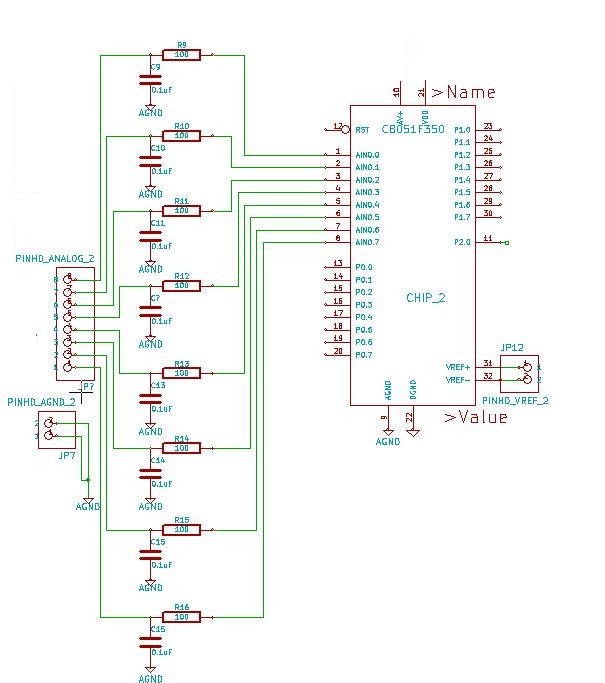
\includegraphics[width=1.10\textwidth, height = 9cm]{esquematicoFiltro2}
  \caption{Esquemático del Circuito Completo de entradas analogicas.}\label{fig:esquematicoFiltro2}
\end{figure}

% subsubsection entradas_analogicas2 (end)

\subsubsection{Circuito de entradas Digitales}
\label{subsub:entradas_digitales}

Como podemos ver en la figura \ref{fig:esquematicoDigital2} colocamos 16 entradas/salidas digitales para el microcontrolador. Cada chip tiene las mismas 16 entradas.

\begin{figure}  [H]
\centering
  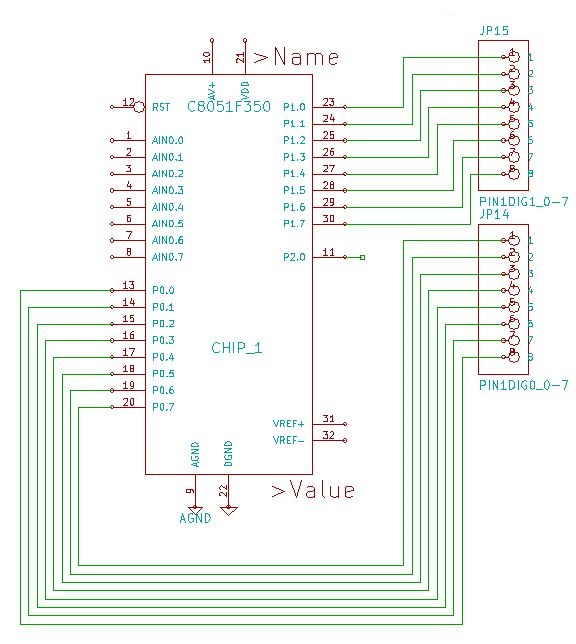
\includegraphics[width=1.0\textwidth, height = 10cm]{esquematicoDigital2}
  \caption{Esquemático del Circuito Completo de entradas/salidas digitales.}\label{fig:esquematicoDigital2}
\end{figure}


% subsubsection entradas_digitales (end)

\subsubsection{Circuito Salida Serial}
\label{subsub:salida_serial2}

La idea de tener una placa a la que se conecten varios sensores analógicos y digitales es que se pueda colocar el lugares remotos, por lo que decidimos que la salida serial deje de ser RS-232 y colocarle dos salidas seriales nivel TTL con un RX y un TX para cada microcontrolador, ademas colocando éste tipo de salida se ahorra mucho espacio, así pudimos reducir el tamaño de la placa. Las salidas seriales se encuentran conectadas directamente en los pines de salidas dijitales P0.4 (Tx) y P0.5(Rx).

% subsubsection salida_serial2 (end)

\subsubsection{Circuito para Debugger y Programación} % (fold)
\label{subsub:debugger_programacion2}

Para programar cada uno de los microcontroladores en principio se penso en colocar dos entradas para el debugger de SiliconLabs, pero nos consumia mucho espacio y el cambio para programar uno y otro se hubiera hecho molesto. Por lo que decidimos poner uno solo, y utilizarlo para los dos microcontroladores, con un jumper de tres pines, para tener la opcion de elegir que micro programar.
En la figura \ref{fig:esquematicoDebugger2} vemos en uno de los C8051f352 como queda conectado el modulo de debugger/programacion.

\begin{figure}  [H]
\centering
  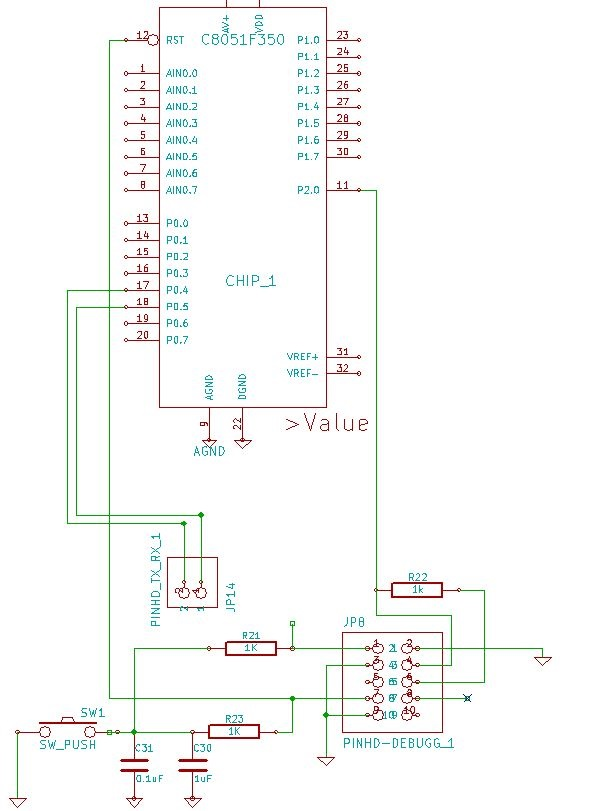
\includegraphics[width=1.0\textwidth, height = 8cm]{esquematicoDebugger2}
  \caption{Esquemático del Circuito para la programacion de los microcontroladores de la placa.}\label{fig:esquematicoDebugger2}
\end{figure}


% subssubection debugger_programacion2 (end)

\subsubsection{Circuito de Potencia}
\label{subsub: circuito_potencia2}

Para el circuito de potencia hicimos lo mismo que con el debugger, colocamos una sola entrada y un solo regulador para toda la placa y alimentar asi los dos microcontroladores. Tambien colocamos un jumpers (JMP3), se utiliza para decidir si alimentamos la placa con una fuente externa o con el debugger/programador de SiliconLabs. 
Sabemos que el principal problema de un sitema embebido es su consumo de energia, por lo que colocamos dos jumpers más, uno para cada una de las entradas de alimentación del segundo microcontroladore (JP4 AV+ y JP5 para VDD). Entonces así podemos elegir desconectar un chip y ahorrar el consumo de energia que este provocaría. 

En la figura \ref{fig:esquematicoPotencia2} se muestra como queda el esquematico del circuito de potencia.

\begin{figure}[H] 
\centering
  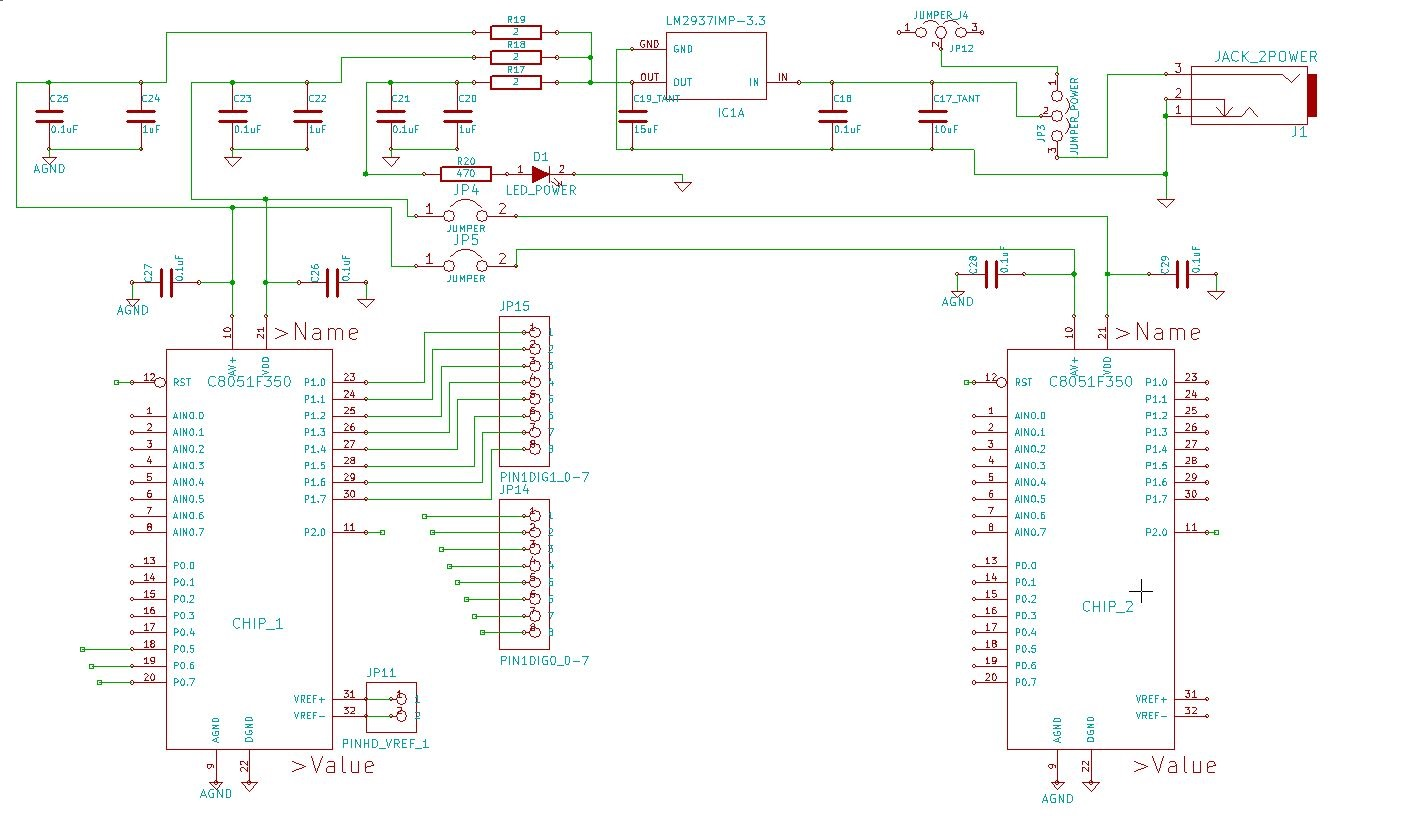
\includegraphics[width=1.0\textwidth, height = 10cm]{esquematicoPotencia2}
  \caption{Esquemático del Circuit para la potencia de alimentación.}\label{fig:esquematicoPotencia2}
\end{figure}

%subsubsection circuito_potencia2 (end)

\subsubsection{Diagrama Esquematico Completo}
\label{subsubsection: esquematico_completo2}

En la figura \ref{fig:esquematicoCompleto2} podemos ver como queda el esquematico entero con los dos microcontroladores y todos los subcircuitos que componen la placa.

\begin{figure}  
\centering
  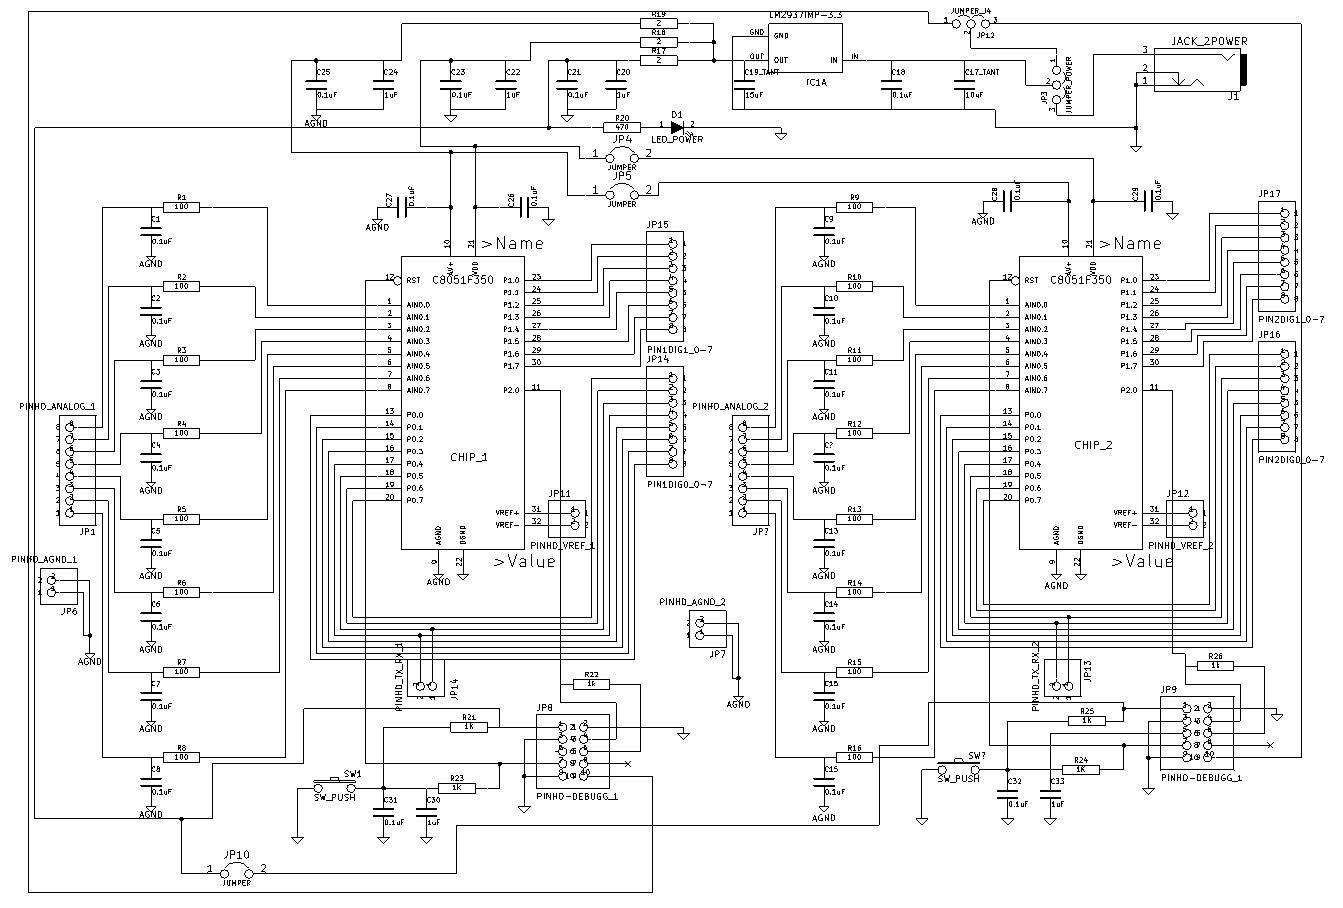
\includegraphics[width=1.10\textwidth, height = 12cm]{esquematicoCompleto2}
  \caption{Esquemático del Circuit completo de la Placa de desarrollo.}\label{fig:esquematicoCompleto2}
\end{figure}


% subsubsection esquematico_completo2 (end)

% subsection diseño_esquematico2 (end)

\subsection{Diseño de Plaqueta de Circuito Impreso (PCB)}
\label{ subsection: diseño_pcb2}

Como esta nueva version de la placa fue diseñada para ser doble capa, se mostrarán 2 figuras, una para la capa superior y otra para la capa inferior. 
A ambas capaz le tuvimos que dividir las masas, en una seccion analogica y una digital, la masa analogica de la capa superior con la de la capa inferior deben estar interconectadas, lo mismo pasa con la masa digital. Por lo que realizamos un drill (un hueco) para que las masas esten en contacto.
En la figura \ref{fig:PCB2a} podemos ver como queda el diagrama PCB de capa superior o frontal, y en la figura \ref{fig:PCB23Da} vemos la misma capa con el visualizador 3D del KiCad.

\begin{figure}[H]
\centering
  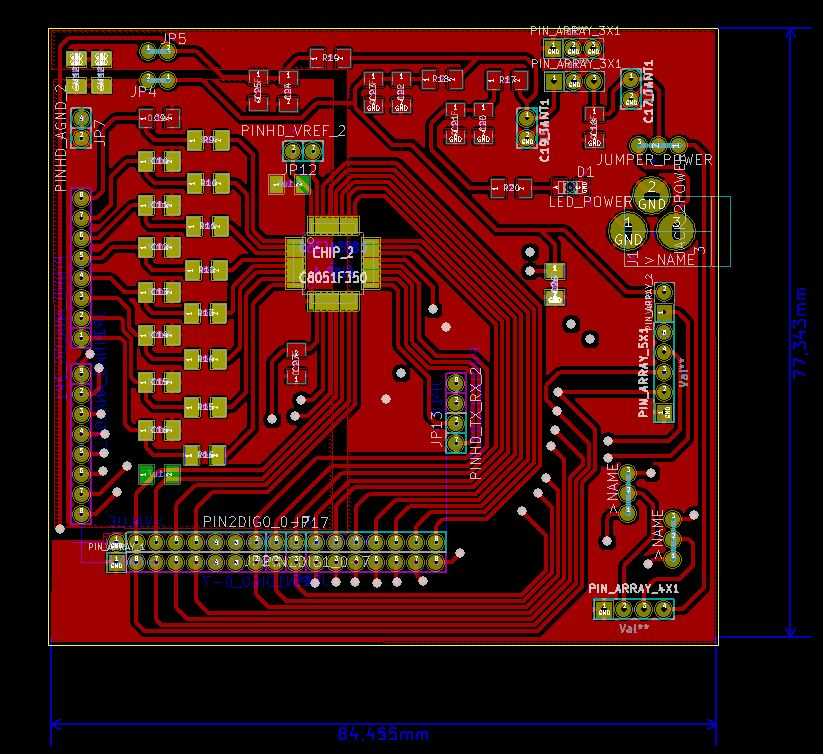
\includegraphics[width=1.0\textwidth, height = 8cm]{PCB2a}
  \caption{Diseño PCB de la capa frontal de la placa.}\label{fig:PCB2a}
\end{figure}

\begin{figure}  [H]
\centering
  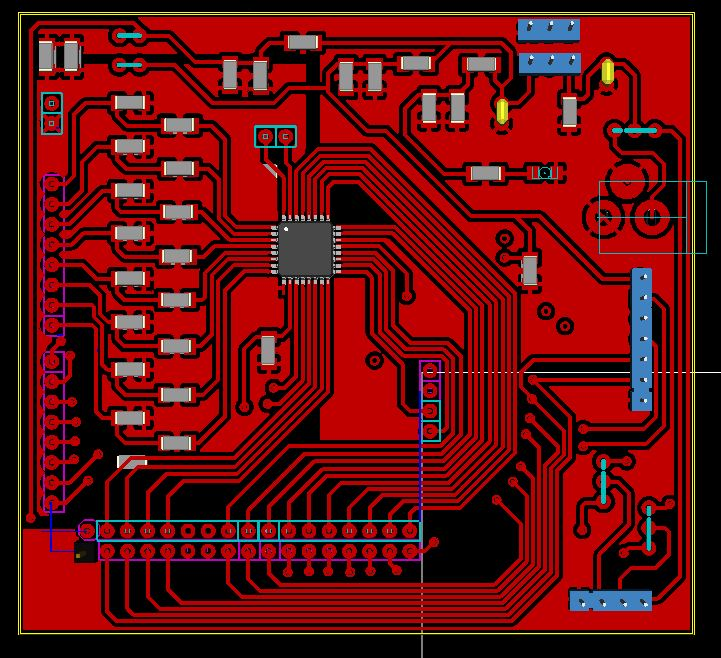
\includegraphics[width=1.0\textwidth, height = 8cm]{PCB23Da}
  \caption{Diseño PCB de la capa frontal de la placa en 3D.}\label{fig:PCB23Da}
\end{figure}

En la figura \ref{fig:PCB2b} podemos ver como queda el diagrama PCB de capa inferior o posterior, y en la figura \ref{fig:PCB23Db} vemos la misma capa con el visualizador 3D del KiCad.

\begin{figure}[H] 
\centering
  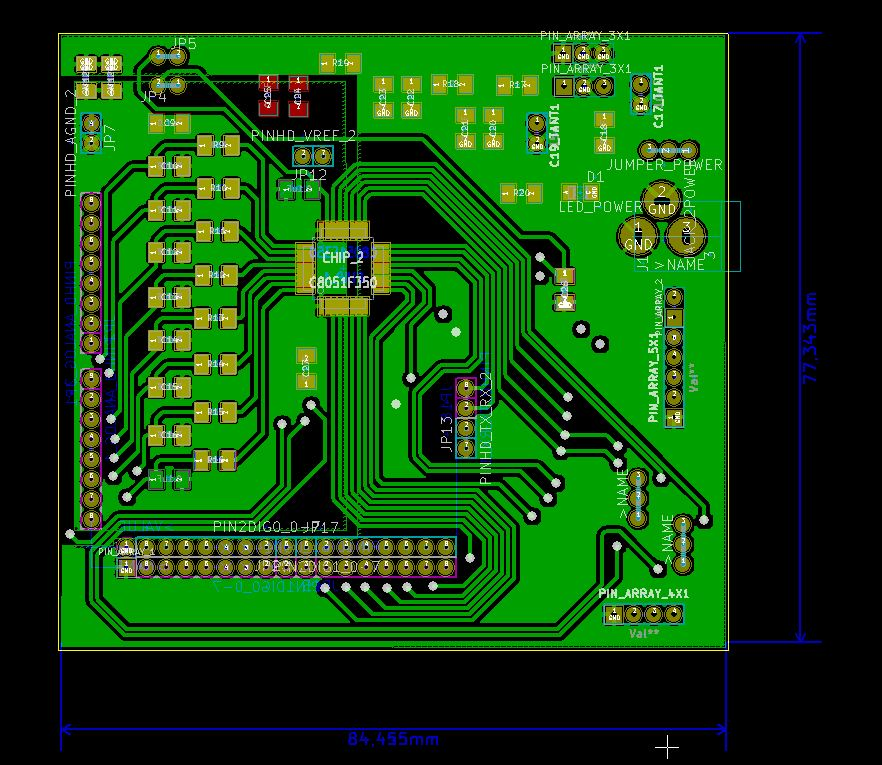
\includegraphics[width=1.0\textwidth, height = 8cm]{PCB2b}
  \caption{Diseño PCB de la capa posterior de la placa.}\label{fig:PCB2b}
\end{figure}

\begin{figure}  [H]
\centering
  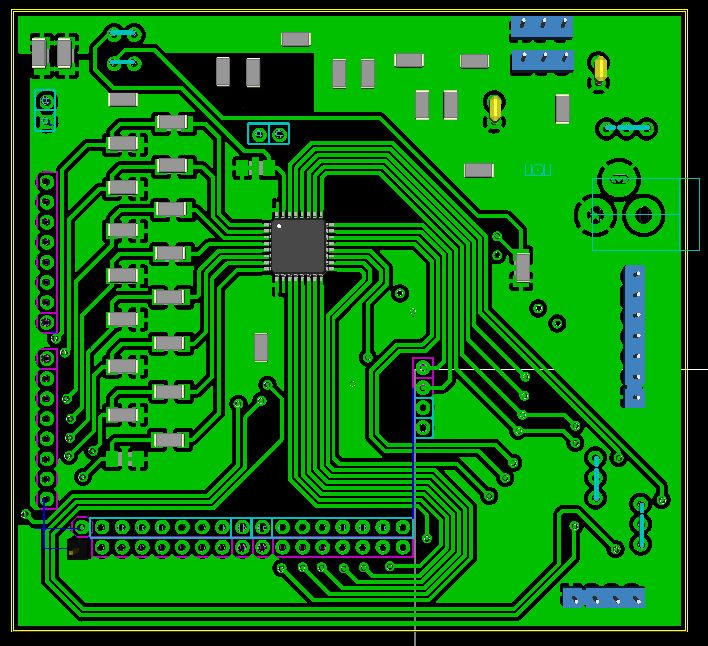
\includegraphics[width=1.0\textwidth, height = 8cm]{PCB23Db}
  \caption{Diseño PCB de la capa posterior de la placa en 3D.}\label{fig:PCB23Db}
\end{figure}


% subsection diseño_pcb2 (end)

\section{Pruebas} % (fold)
\label{sec:pruebas}

En la tabla de pruebas se veran repetidos los mismos tests que en la iteracion anterior, ya que fue necesario que los realicemos nuevamente. La diferencia se encuentran en los resultados.

\begin{table}[h]
\caption{Test de sistema 1}
\label{it4:tab:testsistema1}
\begin{tabular}{p{2cm} p{9cm}}
\multicolumn{2}{c}{\cellcolor[HTML]{68CBD0}{\color[HTML]{000000} Prueba de sistema}} \\
Prueba \#        & 1 \\
\hline
Nombre           & Correcto Diseño de PCB. \\
\hline
Requerimientos  &  \tabitem La placa debe tener dos microcontroladores C8051f352. \\
                &  \tabitem La placa debe tener 16 entradas analogicas. \\
                &  \tabitem La placa debe tener 32 entradas digitales. \\
                &  \tabitem La placa debe tener 2 salidas seriales.   \\
\hline
Descripción      & Se chequea si existen errores en el diseño utilizando el ERC (perfom design rules check) que provee KiCad. \\
\hline
Pre-condiciones  & \tabitem Componentes colocados y ruteados. \\
                 & \tabitem Pads numerados con sus etiquetas.  \\
\hline
Post-condiciones & El resultado de ERC debe ser cero. \\
\hline
Resultados       & No encontramos errores de diseño en el PCB. \\                                                                           
\end{tabular}
\end{table}

\begin{table}[h]
\caption{Test de sistema 2}
\label{it4:tab:testsistema2}
\begin{tabular}{p{2cm} p{9cm}}
\multicolumn{2}{c}{\cellcolor[HTML]{68CBD0}{\color[HTML]{000000} Prueba de sistema}} \\
Prueba \#        & 2 \\
\hline
Nombre           & Correcta impresión de la placa.   \\

\hline
Requerimientos &    \tabitem La placa debe tener dos microcontroladores C8051f352. \\
               &    \tabitem La placa debe tener 16 entradas analogicas.\\
               &    \tabitem La placa debe tener 32 entradas digitales. \\
               &    \tabitem La placa debe tener 2 salidas seriales.    \\
\hline
Descripción      & Corroboramos que todas las pistas y que todos los drills se hayan impreso. Luego con un multimetro seteado en continuidad comprobamos que no existan cortocircuitos entre pistas y masa o entre pads y masa. \\
\hline
Pre-condiciones  & \tabitem Placa impresa. \\
                 & \tabitem Multímetro seteado en continuidad. \\
\hline
Post-condiciones & La placa debe tener las mismas pistas que aparecen en el diseño de PCB, y al medir con el tester nunca debe dar continuidad entre masa y pistas, o entre pads y pistas. \\ 
\hline
Resultados       & Todas las pistas estaban de acuerdo con el PCB. Al medir la continuidad de las pistas no se encontraron a cortocircuitos. \\                                                                                                                                     
\end{tabular}
\end{table}

\begin{table}[h]
\centering
\caption{Test de sistema 3}
\label{it4:tab:testsistema3}
\begin{tabular}{p{2cm} p{9cm}}
\multicolumn{2}{c}{\cellcolor[HTML]{68CBD0}{\color[HTML]{000000} Prueba de sistema}} \\
Prueba \#        & 3 \\
\hline
Nombre           & Correcta soldadura de Componentes. \\
\hline
Requerimientos &    \tabitem La placa debe tener dos microcontroladores C8051f352. \\
               &    \tabitem La placa debe tener 16 entradas analogicas. \\
               &    \tabitem La placa debe tener 32 entradas digitales. \\
               &    \tabitem La placa debe tener 2 salidas seriales.      \\
\hline
Descripción      & Se utiliza el multimetro seteado en continuidad para poder chequear si existen cortocircuitos y para saber si todos los componentes estan bien interconectados. \\
\hline
Pre-condiciones  & \tabitem Placa impresa. \\
                 & \tabitem Pistas impresas correctamente. \\
                 & \tabitem Componentes soldados. \\
                 & \tabitem Multimetro seteado en continuidad. \\
\hline
Post-condiciones &  No deben encontrarse cortocircuitos, y deben comprobarse la continuidad de las interconexiones de componentes. \\ 
\hline
Resultados       & Encontramos cortocircuitos luego de soldar los componentes, se solucionaron desoldando y volviendo a soldar los componentes. \\                                                                                                                                             
\end{tabular}
\end{table}

\begin{table}[h]
\centering
\caption{Test de sistema 4}
\label{it4:tab:testsistema4}
\begin{tabular}{p{2cm} p{9cm}}
\multicolumn{2}{c}{\cellcolor[HTML]{68CBD0}{\color[HTML]{000000} Prueba de sistema}} \\
Prueba \#        & 4 \\
\hline
Nombre           & Correcta Comunicación Con IDE SiliconLabs. \\
\hline
Requerimientos &  \tabitem Se debería poder conectar el debugger del microcontrolador a la placa para poder programarlo. \\
\hline
Descripción      & Se utilizo el cable USB con el debugger de SiliconLabs para conectar la placa a la PC. \\
\hline
Pre-condiciones  & \tabitem Placa impresa. \\
                 & \tabitem Pistas impresas correctamente. \\
                 & \tabitem Componentes soldados. \\
                 & \tabitem IDE SiliconLabs instalada en la PC. \\
\hline
Post-condiciones &  Al abrir la IDE y apretar el botón de "Connect" el programa debe reconocer el tipo de microcontrolador al que esta conectado. \\ 
\hline
Resultados       &  Conectamos la placa a la PC y en la IDE apretamos el botón de conectar, con lo que nos reconoció que el micro que se había conectado fue un C8051f352.     \\                                                                                                                                               
\end{tabular}
\end{table}

\begin{table}[h]
\centering
\caption{Test de sistema 5}
\label{it4:tab:testsistema5}
\begin{tabular}{p{2cm} p{9cm}}
\multicolumn{2}{c}{\cellcolor[HTML]{68CBD0}{\color[HTML]{000000} Prueba de sistema}} \\
Prueba \#        & 4 \\
\hline
Nombre           & Correcta programacion del microcontrolador. \\
\hline
Requerimientos &  \tabitem Se debería poder conectar el debugger del microcontrolador a la placa para poder programarlo. \\                                   
\hline
Descripción      & Se utilizo el cable USB con el debugger de SiliconLabs para conectar la placa a la PC y descargarle un programa .hex al microcontrolador. \\
\hline
Pre-condiciones  & \tabitem Placa impresa. \\
                 & \tabitem Pistas impresas correctamente. \\
                 & \tabitem Componentes soldados. \\
                 & \tabitem IDE SiliconLabs instalada en la PC. \\
                 & \tabitem IDE SiliconLabs reconociendo el C8051f352. \\
\hline
Post-condiciones &  Al abrir la IDE y apretar el botón de "Connect" el programa debe reconocer el tipo de microcontrolador al que esta conectado y luego a traves de la misma IDE o del "Flash Programing Utilitys" cargarle un proframa .hex al c8051f352. \\ 
\hline
Resultados       &  Conectamos la placa a la PC y desde el "Flash Programing Utilitys" se pudo cargar un programa a los microcontroladores soldados en la placa. \\                                                                                                  
\end{tabular}
\end{table}

\begin{table}[h]
\centering
\caption{Test de sistema 6}
\label{it4:tab:testsistema6}
\begin{tabular}{p{2cm} p{9cm}}
\multicolumn{2}{c}{\cellcolor[HTML]{68CBD0}{\color[HTML]{000000} Prueba de sistema}} \\
Prueba \#        & 4 \\
\hline
Nombre           & Correcta funcionamiento de las entradas analogicas y salidas digitales. \\                      

\hline
Requerimientos &    \tabitem La placa debe tener dos microcontroladores C8051f352. \\
               &    \tabitem La placa debe tener 32 entradas digitales. \\
               &    \tabitem La placa debe tener 16 entradas analogicas. \\
\hline
Descripción      & Cargamos un programa a los microcontroladores con el que medimos una entrada analogica proveniente de una fuente (prestada en el Pañol) y utilizamos el ADC para poder transformar esa señal analogica en digital, luego en una de las salidas/entradas digitales se conecto un led, el cual titilaria con mayor frecuencia a medida que se aumenta el voltage que entrega la fuente utilizada. \\
\hline
Pre-condiciones  & \tabitem Placa impresa. \\
                 & \tabitem Pistas impresas correctamente. \\
                 & \tabitem Componentes soldados. \\
                 & \tabitem IDE SiliconLabs instalada en la PC. \\
                 & \tabitem IDE SiliconLabs reconociendo el C8051f352. \\
                 & \tabitem Programa de prueba correctamente cargado en el C8051f352. \\
                 & \tabitem Fuente de Tension externa conecectada a las entradas analogicas con referencia en masa analogica. \\
                 & \tabitem Resistencia conectada en serie con un Led a una salida digital del C8051f352. \\
\hline
Post-condiciones &  Al apregar el boton de "Go" en el "Flash Programing Utilitys" para que arranque a funcionar el programa cargado en el microcontrolador debe titilar el led variando su frecuencia en directa relacion con la variacion de la tension de la fuente conectada a las entradas analogicas. \\ 
\hline
Resultados       &  Cargamos el programa en el microcontrolador, y con todas las pre-condiciones cumplidas hicimos correr el programa. El led efectivamente vario su frecuencia de prendido y apagado a medida que aumentabamos o disminuiamos la tension que entregaba la fuente externa. \\                                                                                                            
\end{tabular}
\end{table}


% section pruebas (end)

\section{Resultados} % (fold)
\label{sec:resultados}

Cumplimos con los requerimientos planteados para esta iteracion:

\begin{itemize}
  \item La placa debe tener dos microcontroladores C8051f352.
  \item La placa debe tener 16 entradas analogicas.
  \item La placa debe tener 32 entradas digitales.
  \item La placa debe tener 2 salidas seriales. 
  \item Se debería poder conectar el debugger del microcontrolador a la placa para poder programarlo.
\end{itemize}


 Obtivimos una placa de desarrollo que dobla en recursos a la placa de la iteración anterior. La placa quedó totalmente funcional.
En la figura \ref{fig:} y \ref{fig:} podemos ver como quedo la placa tanto de la capa superior como de la inferior. Lo que observamos es que todos los pines y modulos que se pueden utilizar para conectar alguna interfaz/cable quedaron en la capa frontal, por una cuestion de comodidad al momento de utilizarla.

"AGREGAAAAAAAAAAAAAAAAAR LAS FOTTTOOOOOOOOOOOOOOOOOOOOOOOOOOOOOOOOOOOOOOOOOOOOOOOOOOOOOOOOOOS"

% section resultados (end)

% chapter iteracion_4 (end)